\documentclass[border=4pt]{standalone}
% Preámbulo común de las figuras. Cada figura es un documento standalone
% que se compila a SVG con scripts/build_figures.sh
\usepackage[utf8]{inputenc}
\usepackage{amsmath}
\usepackage{tikz}
\usepackage[american, siunitx]{circuitikz}
\usetikzlibrary{arrows.meta,calc,decorations.pathmorphing,patterns}
\tikzset{
  >={Stealth[length=2.2mm]},
  eje/.style={->, thin},
  hilo/.style={thick},
}
% Paleta común: tonos medios legibles sobre fondo claro
\definecolor{azul}{RGB}{31,94,168}
\definecolor{rojo}{RGB}{192,57,43}
\definecolor{verde}{RGB}{39,128,73}
\definecolor{naranja}{RGB}{211,120,30}
\definecolor{morado}{RGB}{125,60,152}

\begin{document}
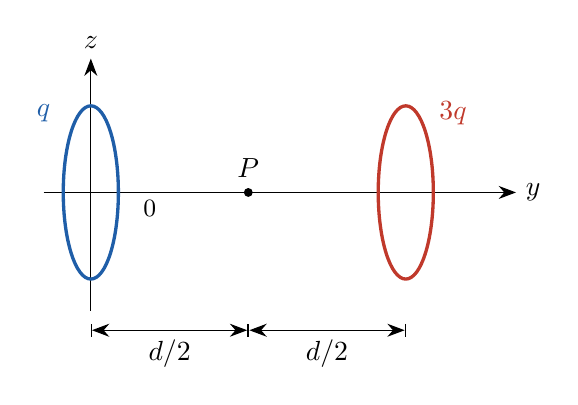
\begin{tikzpicture}[scale=1.0]
  \draw[eje] (-0.6,0) -- (5.4,0) node[right]{$y$};
  \draw[eje] (0,-1.5) -- (0,1.7) node[above]{$z$};
  \draw[very thick, azul] (0,0) ellipse (0.35 and 1.1);
  \draw[very thick, rojo] (4,0) ellipse (0.35 and 1.1);
  \node[azul] at (-0.6,1.0) {$q$};
  \node[rojo] at (4.6,1.0) {$3q$};
  \fill (2,0) circle (1.6pt) node[above=2pt]{$P$};
  \draw[|<->|, thin] (0,-1.75) -- node[below]{$d/2$} (2,-1.75);
  \draw[|<->|, thin] (2,-1.75) -- node[below]{$d/2$} (4,-1.75);
  \node[font=\small] at (0.75,-0.2) {$0$};
\end{tikzpicture}
\end{document}
